\documentclass{article}
\usepackage[utf8]{inputenc}
\usepackage{amsmath}
\usepackage{amsfonts}
\usepackage{amssymb}
\usepackage{hyperref}
\usepackage{tikz}
\usepackage{graphicx} % Required for including images
\usepackage{float} % For precise placement of figures
\usepackage{booktabs} % For formal tables
\usepackage{listings} % For code listing

% Configuration de l'apparence du code
\lstset{
    basicstyle=\footnotesize\ttfamily,
    breaklines=true,
    frame=single,
    numbers=left,
    numberstyle=\tiny\color{gray},
    showstringspaces=false,
    tabsize=2
}

\title{Virothérapie dans le traitement du cancer}
\author{Dan, Martin, Hugo}
\date{\today}

\begin{document}

\maketitle

\section{État de l'art}

Les virus oncolytiques, conçus spécifiquement pour cibler les cellules cancéreuses, rencontrent des mécanismes de résistance qui peuvent réduire leur efficacité \cite{goradel2022}. La compréhension de ces mécanismes est cruciale pour améliorer les stratégies thérapeutiques actuelles. Les recherches indiquent que les virus oncolytiques peuvent être utilisés efficacement dans différentes approches thérapeutiques, y compris en combinaison avec la chimiothérapie pour traiter divers types de cancer \cite{zeyaullah2012}.

Les défis liés à la sélection du virus et de la plateforme génétique appropriés sont importants. La sélection du virus idéal pour une thérapie donnée implique de prendre en compte la biologie du virus, la spécificité tumorale et la capacité de porter des gènes thérapeutiques \cite{mcfadden2021}. De plus, la réponse immunitaire anticancéreuse varie considérablement entre les modèles animaux et humains, ce qui complique la prédiction de l'efficacité des traitements à base de virus oncolytiques chez l'homme.

Enfin, l'utilisation de virus oncolytiques en tant qu'adjuvants pour la vaccination anticancéreuse personnalisée représente une autre approche innovante. Cette stratégie, actuellement en phase de test clinique, utilise deux virus différents exprimant le même antigène tumoral pour amorcer et renforcer l'immunité antitumorale \cite{roy2021}. L'efficacité de cette vaccination dépend en partie de la sensibilité variable de chaque tumeur à l'infection par le virus oncolytique.

La virothérapie en oncologie est un domaine en pleine expansion, avec des progrès significatifs et des défis persistants. La compréhension approfondie des interactions entre les virus, les tumeurs et le système immunitaire est essentielle pour optimiser cette forme de traitement et la rendre plus efficace.

\section{Modèle de virothérapie}
Dans cette partie, on détaille un modèle mathématique de virothérapie, qui utilise des équations différentielles ordinaires pour décrire la dynamique entre les cellules tumorales et les particules virales oncolytiques.

\subsection{Hypothèses du Modèle}
Le modèle repose sur plusieurs hypothèses :
\begin{itemize}
  \item Les populations de cellules et de virus sont bien mélangées et uniformément distribuées.
  \item Les taux de croissance, d'infection et de mort sont constants au cours du temps.
  \item Les interactions virus-cellule sont instantanées et ne dépendent que de la présence et de la densité des populations respectives.
  \item L'environnement tumoral est fermé, sans introduction ou élimination externe de cellules ou de virus, à l'exception de la mort cellulaire et de la clairance virale.
\end{itemize}

\subsection{Analyse des Équations Différentielles}
Le modèle considère trois populations principales: les cellules tumorales non infectées \( x(t) \), les cellules tumorales infectées \( y(t) \), et les particules virales libres \( v(t) \). Les équations suivantes régissent la dynamique du système :

\begin{align}
    \frac{dy}{dt} &= ry\left[1 - \left(\frac{y + x}{K}\right)^\epsilon\right] - kyv - \rho xy, \\
    \frac{dx}{dt} &= kyv - \delta x, \\
    \frac{dv}{dt} &= \alpha x - \omega v - kyv.
\end{align}

\subsubsection{Interprétation des Termes}
\begin{itemize}
  \item \( ry\left[1 - \left(\frac{y + x}{K}\right)^\epsilon\right] \) représente la croissance logistique des cellules infectées, modulée par la capacité porteuse \( K \) et l'effet de la densité de population contrôlé par l'exposant \( \epsilon \).
  \item \( kyv \) décrit l'infection des cellules tumorales non infectées par les particules virales, avec \( k \) étant le taux d'infection.
  \item \( \rho xy \) représente la formation de syncytia à partir des cellules infectées et non infectées, ce qui peut conduire à une augmentation de la destruction cellulaire.
  \item \( \delta x \) est le taux de mort naturelle des cellules tumorales non infectées.
  \item \( \alpha x \) indique la production de nouvelles particules virales par les cellules infectées.
  \item \( \omega v \) est le taux d'élimination des particules virales par des mécanismes tels que la clairance immunitaire ou la dégradation naturelle.
\end{itemize}

\subsection{Paramètres du Modèle et Détermination}
Nous présentons maintenant les paramètres du modèle dans le tableau ci-dessous, avec leur signification biologique et la méthode de détermination :

\begin{table}[h]
\centering
\resizebox{\textwidth}{!}{
\begin{tabular}{@{}lll@{}}
\toprule
\textbf{Paramètre} & \textbf{Description}                                          & \textbf{Détermination}                                  \\ \midrule
\( r \)            & Taux de croissance des cellules infectées                     & Ajustement des courbes de croissance cellulaire         \\
\( K \)            & Capacité porteuse de l'environnement tumoral                  & Taille maximale de tumeurs observées                    \\
\( k \)            & Taux d'infection des cellules par les virus                   & Essais virologiques quantitatifs                        \\
\( \delta \)       & Taux de mort naturelle des cellules non infectées             & Études de survie cellulaire                             \\
\( \rho \)         & Taux de formation de syncytia                                & Observation de la fusion cellulaire                     \\
\( \alpha \)       & Taux de production de virus par cellule infectée              & Quantification des virions produits                     \\
\( \omega \)       & Taux d'élimination des virus                                  & Cinétique de dégradation des virus et clairance immunitaire \\
\( \epsilon \)     & Exposant modulant l'effet de la densité de population         & Ajustement aux données de croissance tumorale           \\ \bottomrule
\end{tabular}
}
\caption{Paramètres du modèle de virothérapie et leur méthode de détermination.}
\end{table}

\section{Simulation MATLAB}
Nous avons implémenté un modèle de dynamique de population de virothérapie en utilisant MATLAB. La simulation est basée sur un ensemble d'équations différentielles ordinaires qui modélisent l'interaction entre les cellules tumorales, les cellules infectées par le virus et les particules virales libres.

\subsection{Fonction MATLAB}
La fonction MATLAB suivante a été utilisée pour définir le système d'équations différentielles :

\begin{lstlisting}[language=Matlab, caption={Fonction MATLAB pour la simulation de virothérapie.}, label={lst:matlab_code}]
    function udot = fcn(u)
        r = 0.2062134; % Effective growth rate of uninfected cells day^-1
        K = 2139.258; % Carrying capacity (in 10^6 cells)
        kappa = 0.001; % Infection rate constant (per day per 10^6 cells or virions)
        rho = 0.2145; % Rate constant of cell fusion (per day per 10^6 cells)
        delta = 0.5115; % Effective death rate constant of infected cells day^-1
        omega = 0; % Rate constant of virus elimination day^-1
        alpha = 0; % Virus production rate constant by infected cells (virions per day per cell)
        epsilon = 1.64877; % 
        
        y = u(1); % Tumor cells 
        x = u(2); % Virus infected cell 
        v = u(3); % Free virus cells
        
        ydot = r*y*(1-((y+x)/K).^epsilon)-kappa*y*v-rho*x*y;
        xdot = kappa*y*v - delta*x;
        vdot = alpha*x-omega*v-kappa*y*v;
        
        udot = [ydot, xdot, vdot];
    end
\end{lstlisting}

\subsection{Résultats de Simulation}
La figure \ref{fig:simstate} montre la représentation d'état utilisée dans Simulink pour configurer notre simulation, tandis que la figure \ref{fig:simresult} illustre les résultats de la simulation sous forme de graphiques de la dynamique temporelle des populations.

\begin{figure}[H]
\centering
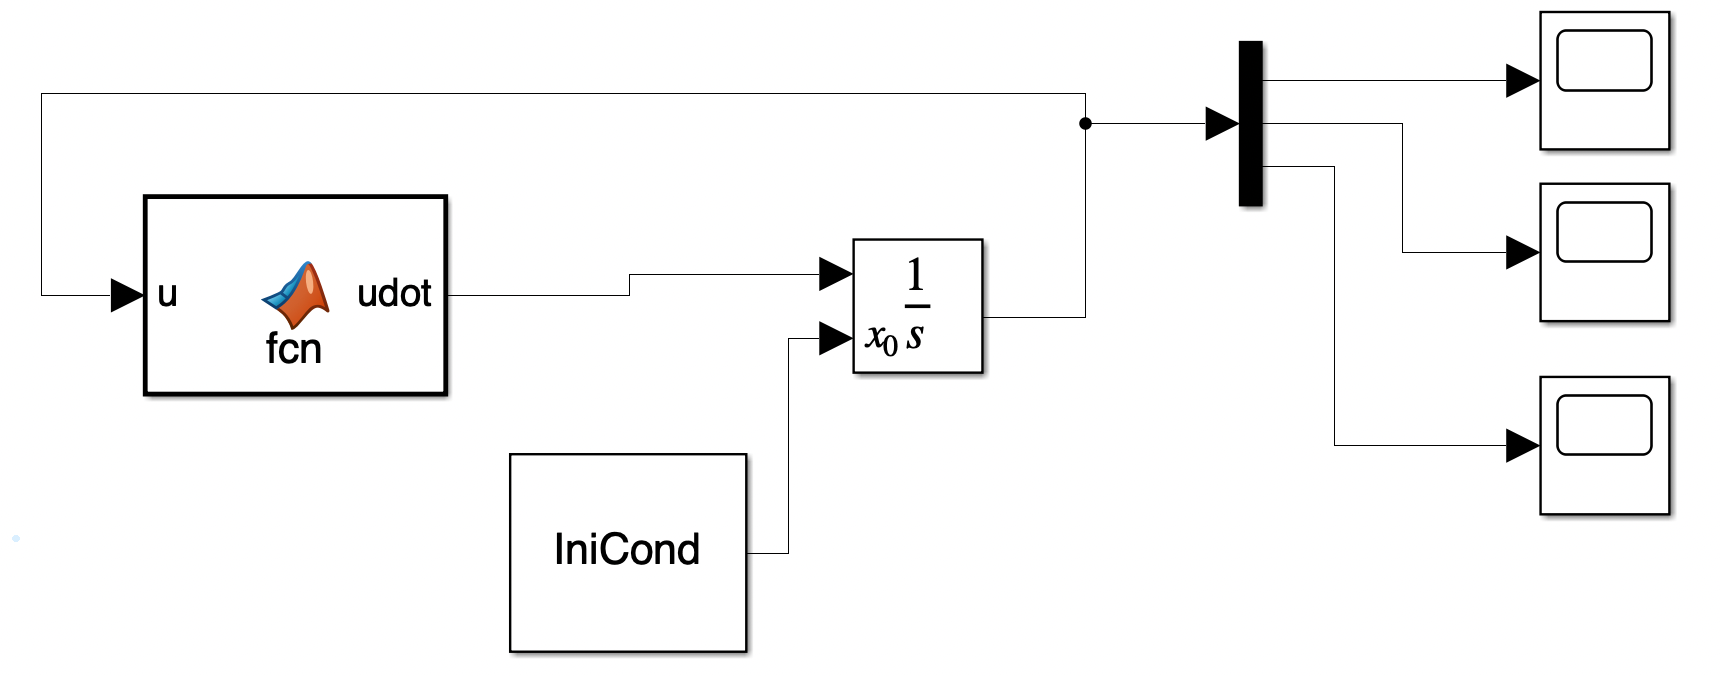
\includegraphics[width=0.8\textwidth]{src/state_representation.png}
\caption{Représentation d'état dans Simulink pour la simulation de virothérapie.}
\label{fig:simstate}
\end{figure}

\begin{figure}[H]
\centering
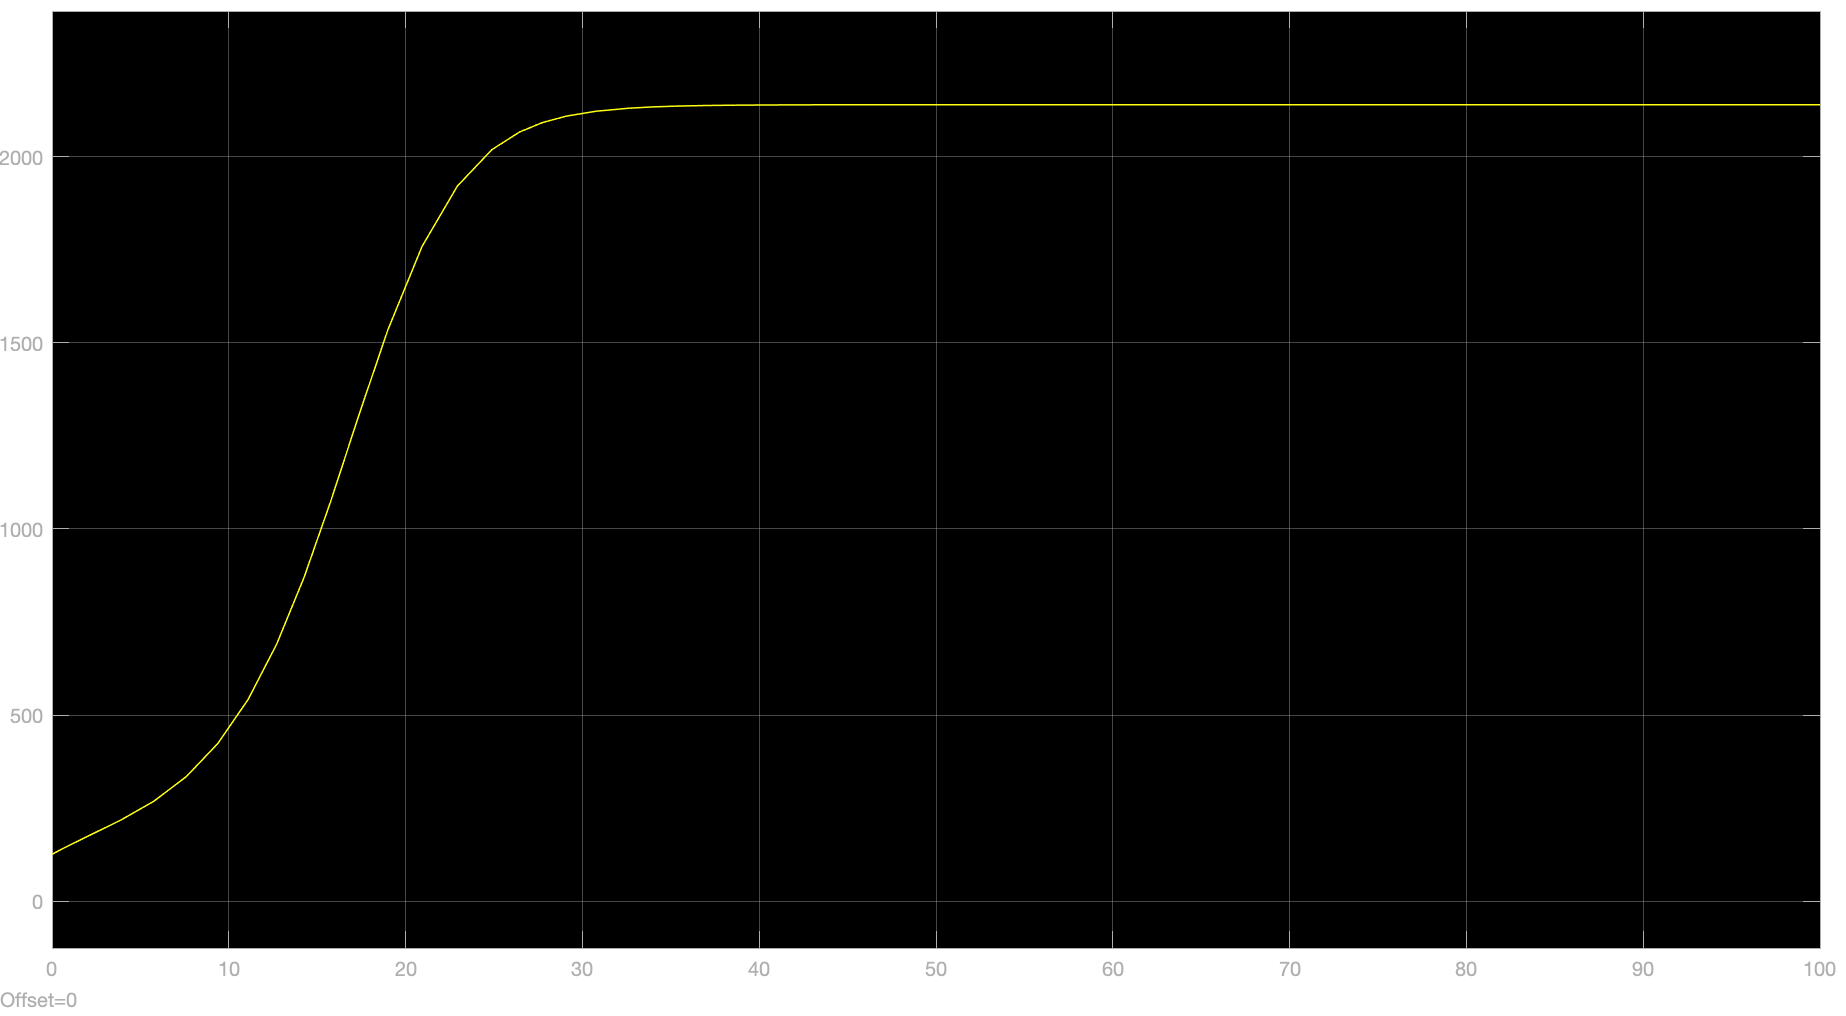
\includegraphics[width=0.8\textwidth]{src/simulation_result.png}
\caption{Résultats de simulation montrant la dynamique des populations.}
\label{fig:simresult}
\end{figure}

\subsection{Paramètres de Simulation}
La table \ref{tab:parameters} récapitule les valeurs des paramètres utilisées pour les simulations.

\begin{table}[h]
    \centering
    \begin{tabular}{@{}cccccccc@{}}
    \toprule
    Variation & \( r \) & \( K \) & \( k \) & \( \delta \) & \( \rho \) & \( \alpha \) & \( \omega \) \\ \midrule
    Base      & 0.0005957 & \( 1 \times 10^6 \) & 0.0001 & 0.1 & 0.0001 & 0.05  & 0.001 \\
    Var 1     & 0.0005957 & \( 1 \times 10^6 \) & 0.0001 & 0.1 & 0.0001 & 0.055 & 0.001 \\
    Var 2     & 0.0005957 & \( 1 \times 10^6 \) & 0.0001 & 0.1 & 0.0001 & 0.06  & 0.001 \\
    Var 3     & 0.0005957 & \( 1 \times 10^6 \) & 0.0001 & 0.1 & 0.0001 & 0.065 & 0.001 \\
    % Continuer avec plus de variations
    \bottomrule
    \end{tabular}
    \caption{Variations des paramètres pour les simulations de virothérapie.}
    \label{tab:parameters}
    \end{table}

\bibliographystyle{unsrt}
\bibliography{references}

\end{document}